% $Id: calculations-substructure.tex 522 2019-04-16 14:42:14Z gsoyez $

%%========================================================================
\chapter{Curiosities: Sudakov Safety}\label{sec:curiosities}
In Chapter~\ref{tools} we have introduced the modified Mass Drop
Tagger/\SD and in Chapter~\ref{calculations-substructure-mass} we have
discussed at length the analytic properties of the jet mass
distribution after mMDT or \SD. Furthermore, we have just analysed
some aspects of applying this grooming technique to jet shapes used
for quark/gluon and W-boson discrimination.
%
However, if we go back to its original definition, we notice that the
\SD condition Eq.~(\ref{eq:soft-drop-condition}) does not involve
directly the jet mass or any jet shape, but rather the distance
between two prongs in the azimuth-rapidity plane $R_{ij}$ and the
momentum fraction
$ z=\tfrac{{\rm min}(p_{t,i},p_{t,j})}{p_{t,i}+p_{t,j}} $. It is quite
natural to ask ourselves if we can apply the calculation techniques
described for jet masses and jet shapes to better characterise the
distributions of these two quantities. To be precise, let us define the
two observables $\theta_g$ and $z_g$ as follows. We start with a jet
which has been re-clustered with Cambridge/Aachen and we apply \SD. When we find the
first declustering with subjets $j_1$ and $j_2$ that passes the \SD
condition Eq.~(\ref{eq:soft-drop-condition}), we define the groomed radius
and the groomed momentum fraction as
\begin{align}\label{eq:thetag-zg-def}
\theta_g& = \frac{R_{12}}{R}, \\
z_g &= \frac{{\rm min}(p_{t,1},p_{t,2})}{p_{t,1}+p_{t,2}},
\end{align}
where $R$ is the original jet radius.
We note that these variables are interesting for a number of
reasons. 
%
The groomed jet radius is of interest because the groomed jet area is
of the order of $\pi \theta_g^2$.  Thus, $\theta_g$ serves as a proxy for the sensitivity of the groomed jet to possible contamination from pileup~\cite{Cacciari:2008gn,Sapeta:2010uk}.
Furthermore, as we shall shortly see, $z_g$ provides us with an almost unique perturbative access to one of the most fundamental building blocks of QCD, namely the Altarelli-Parisi splitting function~\cite{Larkoski:2015lea,Larkoski:2017bvj}.


This last observation has drawn the interest of the scientific
community in particular with the study of heavy-ion collisions. In
particular, an observable such as $z_g$ provides information about how
perturbative QCD evolution is modified by the interaction between the
high-energy jet and the quark-gluon plasma, thus providing a new probe
of the latter.
%
Different experiments have now measured $z_g$ distribution. For
instance the STAR collaboration at the Relativistic Heavy Ion Collider
of the U.S. Brookhaven National Laboratory performed this measurement
using gold-gold collisions~\cite{Kauder:2017mhg}. Furthermore, the CMS
experiment and the ALICE experiments studied this variable, at the
Large Hadron Collider, in lead-lead heavy-ion
collisions~\cite{Chen:2017rhw,Caffarri:2017bmh}. We will describe some
of these measurements in more detail in
Chapter~\ref{searches-measurements}.
%
In parallel, this line of research triggered noticeable interest in
the theoretical nuclear physics and heavy-ion communities,
e.g.~\cite{Lapidus:2017dek,Zapp:2017ria,Tywoniuk:2017dzi,Casalderrey-Solana:2017mjg,Mangano:2017plv,Qin:2017roz,Milhano:2017nzm,Chang:2017gkt,KunnawalkamElayavalli:2017hxo}.

In this chapter, we focus on a baseline description of the $\theta_g$
and $z_g$ observables in proton-proton collision, leaving aside the
extra complications due to interactions of jets with the quark-gluon
plasma in the heavy-ion case.
%
In this context, we anticipate that while we will be able to apply the
standard techniques presented so far in this book in order to obtain a
perturbative prediction for the $\theta_g$ distribution for, the
situation will be very different for $z_g$, where interesting features
emerge.

\section{The groomed jet radius distribution $\theta_g$} \label{sec:thetag}
\begin{figure}[t]
    \centering
    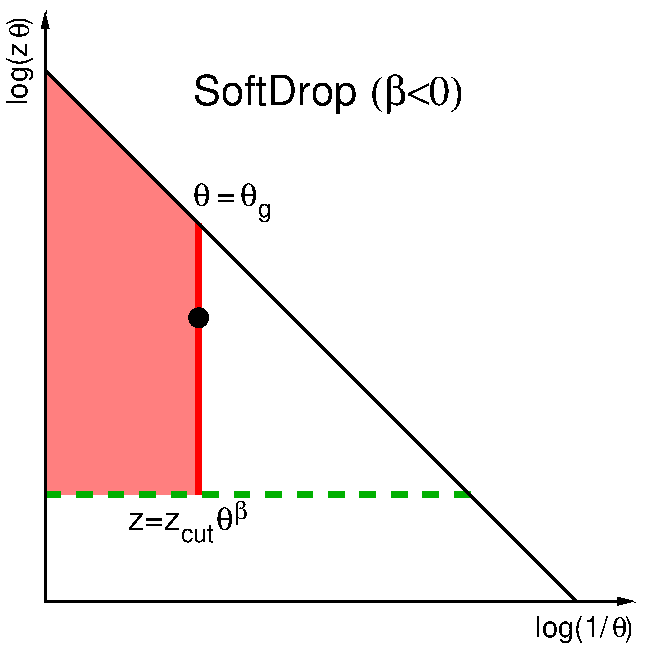
\includegraphics[width=0.32\textwidth]{figures/Lund-SD-thetag-negb.pdf}
    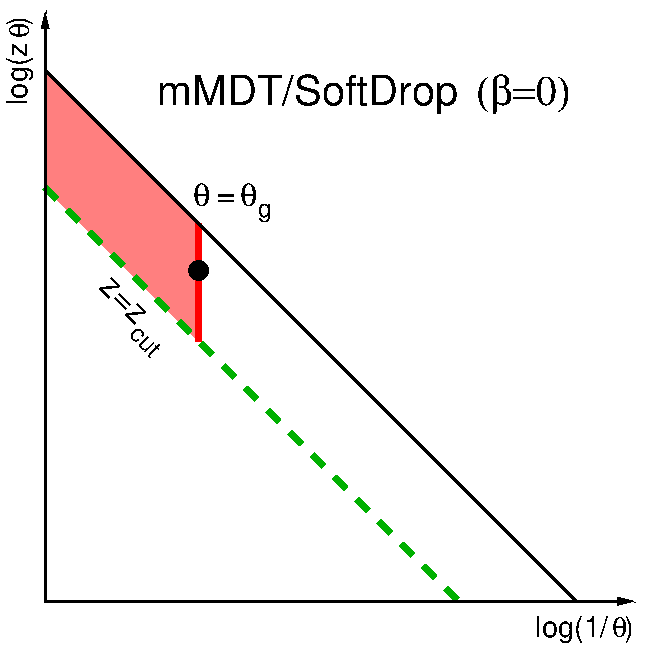
\includegraphics[width=0.32\textwidth]{figures/Lund-SD-thetag-zerob.pdf}
    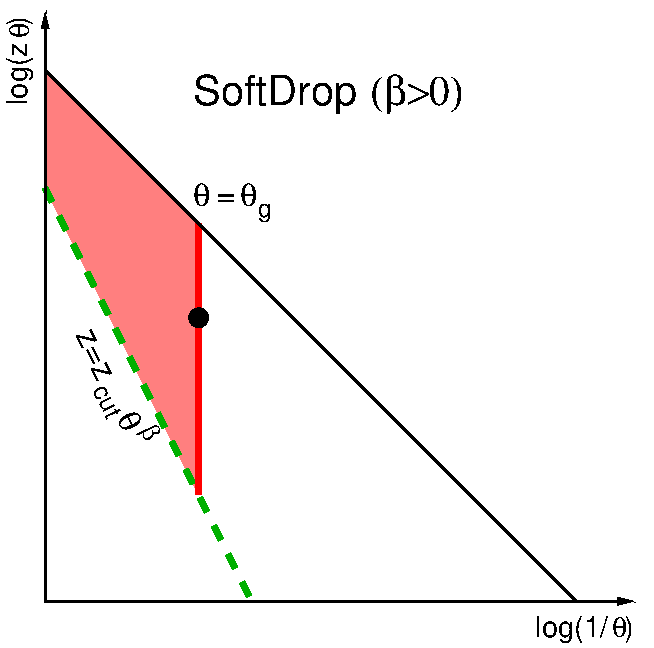
\includegraphics[width=0.32\textwidth]{figures/Lund-SD-thetag-posb.pdf}
  \caption{Lund diagrams for the $\theta_g$ distribution for three representative values of the SD angular exponent $\beta$. From left to right we have $\beta<0$, $\beta=0$ (mMDT) and $\beta>0$. 
  The dashed green line
    represents the edge of SD region, the solid red line corresponds to
    emissions yielding the requested groomed jet radius and the shaded red area is the vetoed area
    associated with the Sudakov suppression. We note that the latter
    is finite in all three cases, as it should be for an IRC
    observable. 
   }\label{fig:lund-sd-thetag}
\end{figure}


We start by calculating the cumulative distribution for the groomed jet radius. In doing so, we are going to exploit the techniques developed in the previous chapters. In particular, we begin by drawing the Lund plane for the observables at hand. We do this in Fig.~\ref{fig:lund-sd-thetag}, where we distinguish three cases according to the sign of the \SD angular exponent $\beta$. From left to right we have $\beta<0$, $\beta=0$ and $\beta>0$. We remind the reader that \SD with $\beta=0$ corresponds to mMDT. 

The dashed green line
    represents the edge of phase-space region where emissions pass the \SD condition, while the solid red line corresponds to
    emissions yielding the requested groomed jet radius. Finally, the
    shaded red area is the region we have to veto in order not to
    exceed the requested groomed radius. With these considerations and
    the expertise gained from the previous chapters, we can almost immediately arrive at an all-order cumulative distribution, which resums leading logarithms and next-to-leading ones but limited to the collinear sector. We have
\begin{equation}\label{eq:grad_exp}
\Sigma_\text{SD}(\theta_g) = \exp\left[
   - \int_{\theta_g}^{1} \frac{d\theta}{\theta}\int_0^{1} dz\, P_{i}(z)\,
   \frac{\alpha_s(z\theta p_tR)}{\pi}
   \Theta\left( z> z_\text{cut}\theta^\beta \right)
\right]\equiv \exp \left[ -R(\theta_g) \right],
\end{equation}
where the integral in the exponent again corresponds to vetoed emissions and $i=q,g$ depending on the jet flavour.
%
We note that the integrals in Eq.~(\ref{eq:grad_exp}) are finite
(modulo the question of the Landau pole) for all values of $\beta$.
%
This is the case because the integral in the exponent arises after adding together real and virtual contributions and therefore its finiteness is guaranteed by the IRC safety of the observable.
%
The integrals in Eq.~(\ref{eq:grad_exp}) can be easily evaluated to
leading-logarithmic accuracy, leading to the following
radiator\footnote{Note that we have used the same approach as for the
  rest of this book and included it in the double-logarithmic
  terms. In this specific case, this is less relevant as the endpoint
  of the distribution does not depend on it, so we could have left it
  explicitly as a separate correction.}
\begin{equation} \label{radiator-rad}
R(\theta_g) 
= \frac{C_i}{2\pi \alpha_s \beta_0^2} \bigg[
     W(1-\lambda_B)
     -W(1-\lambda_g-\lambda_B)
     -\frac{W(1-\lambda_c)}{1+\beta}
     +\frac{W(1-\lambda_c-(1+\beta)\lambda_g)}{1+\beta}\bigg],
   \end{equation}
where $\lambda_g= 2 \as \beta_0 \log\big(\frac{1}{\theta_g}\big)$,
$\lambda_c= 2 \as \beta_0 \log\big(\frac{1}{z_\text{cut}}\big)$ and
$\lambda_B=-2\alpha_s\beta_0B_i$ as before.

For $\beta<0$, this distribution has an
endpoint at $\theta_g^\text{(min)}=\zcut^{-1/\beta}$ (modulo corrections from
hard-collinear splittings). Correspondingly, there is a finite probability,
$\exp[-R(\theta_g^\text{(min)})]$, that the \SD de-clustering
procedure does not find a two-prong structure passing the \SD
condition, in which case we set $\theta_g=0$.

The theoretical calculation is compared to the Monte Carlo prediction,
at parton level, in Fig.~\ref{fig:radius-pythia-v-analytic}, showing
that it captures the main features of the distribution.
%
In particular, we notice that the $\theta_g$ distribution has an
endpoint for negative values of $\beta$, related to the finiteness of
the available phase-space.
%
Furthermore, as $\beta$ decreases, the distribution is shifted towards
smaller angles.\footnote{Here, the case of negative $\beta$ can be seen
  as shifting a whole part of the distribution to
  $\theta_g=0$.} Since the groomed jet area is proportional to
$\pi\theta_g^2$, this agrees with the expectation that smaller $\beta$
corresponds to more aggressive grooming, meaning a smaller jet area or
a smaller sensitivity to pileup and the Underlying Event.


It is
also worth noting that a few complications would arise if we wanted to
extend Eq.~\eqref{radiator-rad} to full NLL accuracy.
% 
Since $\theta_g$ is only sensitive to the first emission being
de-clustered that passes the \SD condition, one could expect that it
does not get any correction from multiple emissions at NLL.
%
However, if one has multiple emissions at a similar angle and
strongly-ordered in energy, which emission emission is de-clustered
first will depend on the details of the Cambridge/Aachen
clustering. This situation, which occurs only for $\beta>0$, is
reminiscent of the non-global and clustering logarithms discussed in
Secs.~\ref{sec:non-global} and \ref{sec:clustering}.
%
This type of effect has been discussed, for instance, in
Refs.~\cite{Neill:2018yet} and~\cite{Dreyer:2018nbf}.

\begin{figure}[t!]
  % 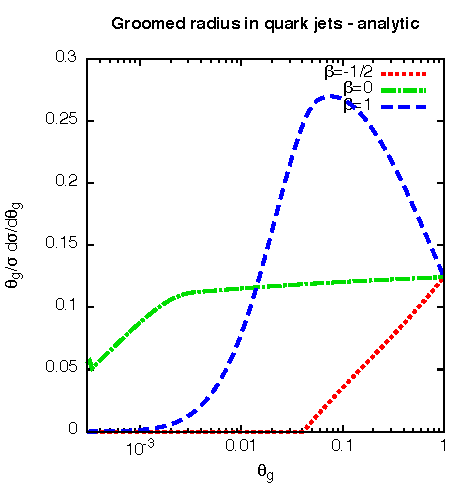
\includegraphics[width=0.49\textwidth,page=1]{figures/sudakov.pdf}
  \centering
  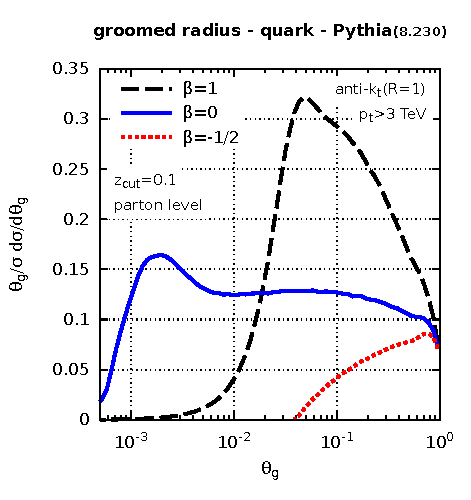
\includegraphics[width=0.48\textwidth,page=1]{figures/zgthetag-pythia.pdf}%
  \hfill%
  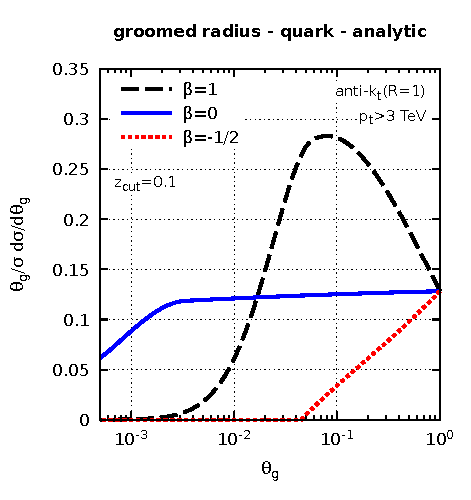
\includegraphics[width=0.48\textwidth,page=1]{figures/zgthetag-analytic.pdf}%
  \caption{The groomed radius distribution The left plot is the result of a Pythia parton-level
    simulation and the right plot is the analytic results discussed in
    this chapter.}\label{fig:radius-pythia-v-analytic}
\end{figure}


\section{The $z_g$ distribution} \label{sec:zg}
\begin{figure}
    \centering
    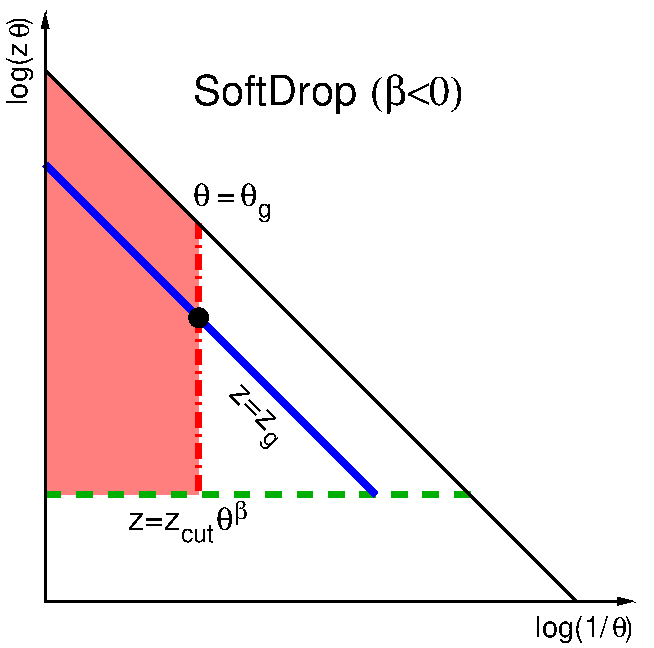
\includegraphics[width=0.32\textwidth]{figures/Lund-SD-zg-negb.pdf}
    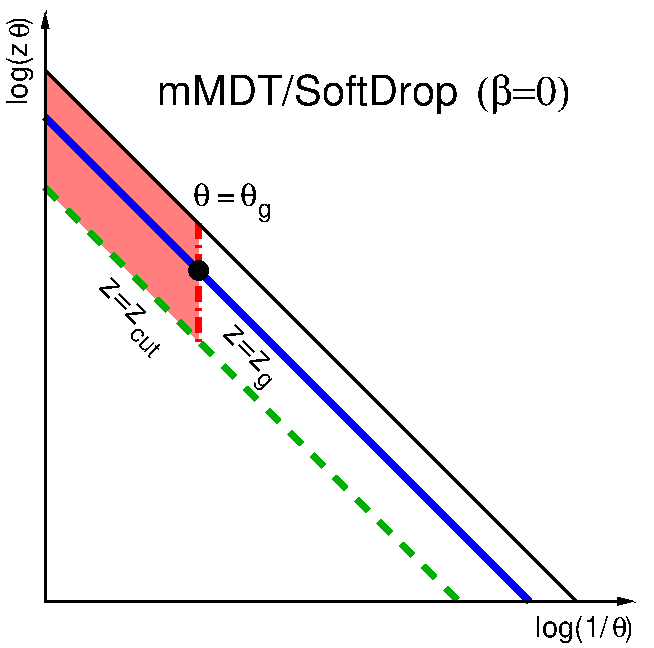
\includegraphics[width=0.32\textwidth]{figures/Lund-SD-zg-zerob.pdf}
    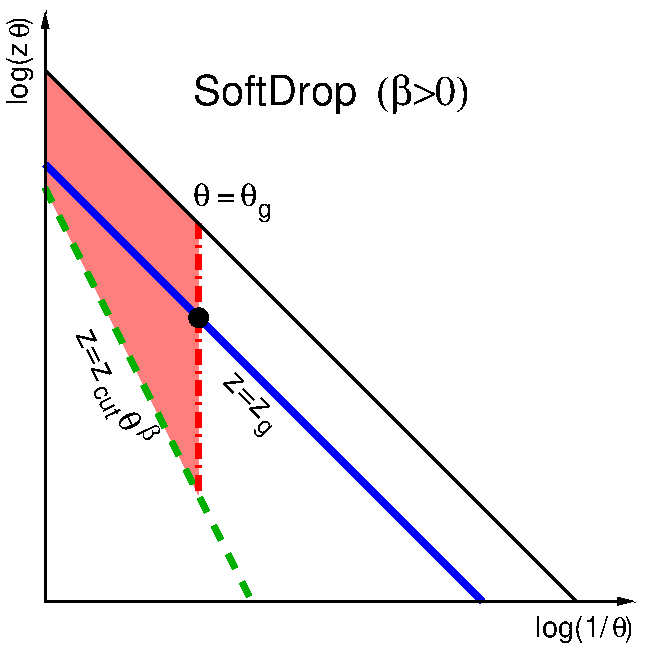
\includegraphics[width=0.32\textwidth]{figures/Lund-SD-zg-posb.pdf}
  \caption{Lund diagrams for the $z_g$ distribution for three representative values of the SD angular exponent $\beta$. From left to right we have $\beta<0$, $\beta=0$ (mMDT) and $\beta>0$. 
  The dashed green line
    represents the edge of SD region
     The dot-dashed red line corresponds to
    emissions yielding a given groomed jet radius and the shaded red area is the vetoed area
    associated with the Sudakov suppression. Finally, the solid blue line corresponds to the requested value of $z_g$. Because we have to integrate over all possible values of $\theta_g$, only the $\beta<0$ case showed on the left exhibits IRC safety.
    %    We note that the latter is finite only when $\beta<0$, while it indefinitely extends in the soft/collinear region when $\beta\ge 0$, signalling the fact that the observable is not IRC safe.  
   }\label{fig:lund-sd-zg}
\end{figure}

We would like now to study the observable $z_g$. This immediately
faces a difficulty: $z_g$ is fixed by the first de-clustering of the
jet that passes the \SD condition. Because we are completely inclusive
over the splitting angle $\theta_g$ we must take into account all
possible values of $\theta_g$ including configurations where the two
prongs become collinear. Indeed collinear splittings always pass the
\SD condition, if $\beta \ge 0$ (strictly speaking, soft-collinear
emissions fail \SD $\beta=0$/mMDT). These configurations are not
cancelled by the corresponding virtual corrections, for which $z_g$ is
undefined, and herald the fact that the observable is not IRC safe.
%
At this point a possible approach would be to just stop this analysis because the observable we are dealing with does not respect the very basic set of properties set out in Chapter~\ref{chap:qcd-colliders}. However, we have just argued that $z_g$ is a very interesting observable for jet substructure and therefore, we decide to be stubborn and push forward with our study. In order to do that, we must generalise the concept of IRC safety and introduce \emph{Sudakov safety}~\cite{Larkoski:2013paa}.
 
 Following~\cite{Larkoski:2015lea}, we introduce a general definition of Sudakov safety which exploits conditional probabilities.
Let us consider an IRC unsafe observable $u$ and a companion IRC safe observable $s$.  The observable $s$ is chosen such that its measured value regulates all singularities of $u$.  That is, even though the probability of measuring $u$,
\begin{equation}
p(u) = \frac{1}{\sigma_0} \frac{d \sigma}{d u},
\end{equation}
is ill-defined at any fixed perturbative order, the probability of measuring $u$ given $s$, $p(u|s)$, is finite at all perturbative orders, except possibly at isolated values of $s$ e.g., $s=0$ for definiteness.  Given this companion observable $s$, we want to know whether $p(u)$ can be calculated in perturbation theory.
%
Because $s$ is IRC safe, $p(s)$ is well-defined at all perturbative
orders and one can define the joint probability distribution
%
\begin{equation}\label{eq:cond_prob}
p(s,u) = p(s)\, p(u|s) ,
\end{equation}
%
which is also finite at all perturbative orders, except possibly at isolated values of $s$.  To calculate $p(u)$, we can simply marginalise over $s$:
%
\begin{equation}
\label{eq:sudsafeone}
p(u) = \int d s\, p(s) \, p(u|s) \,.
\end{equation}
%
If $p(s)$ regulates all (isolated) singularities of $p(u|s)$, thus ensuring that the above integral is finite, then we deem $u$ to be Sudakov safe.

Clearly, we cannot just evaluate $p(s)$ at fixed-order in the strong coupling, but we need some information about its all-order behaviour.  If we consider the resummed distribution for the observable $s$, its distribution will exhibit a Sudakov form factor (hence the name Sudakov safety) that can make the integral in Eq.~(\ref{eq:sudsafeone}) convergent. 
%
In the case that one IRC safe observable is insufficient to regulate all singularities in $u$, we can measure a vector of IRC safe observables $\vec{s}=\{s_1,\dotsc,s_n\}$.  This gives a more general definition of Sudakov safety:
\begin{equation}\label{eq:sudsafedef}
p(u)= \int d^n\vec{s} \, p({\bf s})\, p(u| \vec{s}) \,.
\end{equation}
Only if the vector of safe observables has a finite number of elements, then $u$ is Sudakov safe. For example, particle multiplicity does not fall in this category as it would require an infinite number of safe observables to regulate the arbitrary number of soft/collinear splittings. Thus, particle multiplicity is neither IRC safe, nor Sudakov safe. 


We can now go back to the observable $z_g$ and check whether it is Sudakov safe. To this purpose, we need to introduce a safe companion observable. The \SD procedure itself suggests to use the groomed angle $\theta_g$, which we have calculated in Eq.~(\ref{eq:grad_exp}). 
Therefore, we imagine to measure a value of $z_g$, given a finite angular separation between the two prongs $\theta_g$. This situation is illustrated by the Lund diagrams in Fig.~\ref{fig:lund-sd-zg}. As usual, the dashed green line represents the edge of \SD region. The black dot is the emission passing \SD that provides $z_g$ (solid blue line) and $\theta_g$ (dot-dashed red line). The shaded red area is the vetoed area  associated with the Sudakov suppression for the groomed radius $\theta_g$, i.e.\ it is the same as in Fig.~\ref{fig:lund-sd-thetag}.
%
In order to obtain the $z_g$ distribution, we have to integrate over all possible values of $\theta_g$, which corresponds to all allowed positions for the dot-dashed red line. For $\beta<0$, the area we swipe as we move the red dot-dashed line is bounded by the \SD line in dashed green and it is therefore finite. In this case we expect IRC safety to hold. On the other hand, the $\beta=0$ and $\beta>0$ cases are remarkably different as the resulting area is unbounded. This situation is not IRC safe, but the Sudakov form factor for the groomed radius is enough to regulate (suppress) the resulting divergence. 
We have
\begin{equation}\label{eq:zg-cond-prob}
\frac{1}{\sigma_0}\frac{d \sigma}{d z_g} = \int_0^1 d \theta_g \, p(\theta_g) \, p(z_g|\theta_g),
\end{equation}
where $p(\theta_g)$ is the resummed distribution computed in the
previous section, i.e.\ the derivative of Eq.~(\ref{eq:grad_exp}),
while the conditional probability is calculated at fixed-order in the
strong coupling. In the collinear limit, it reads, for a jet of
flavour $i=q,g$,
\begin{equation}\label{eq:cond-explicit}
p(z_g|\theta_g ) =  \frac{P_{\text{sym},i}(z_g)\as(z_g \theta_g p_t R)}{\int_{z_\text{cut}\theta_g^\beta}^{1/2} d z \, P_{\text{sym},i}(z) \as(z \, \theta_g p_t R)} \Theta(z_g>\zcut \theta_g^\beta)\,,
\end{equation}
where $0 < z_g < 1/2$ and following the approach of Refs.~\cite{Larkoski:2015lea,Larkoski:2017bvj,Tripathee:2017ybi}, we have introduced a symmetrised notation of the splitting function
\begin{equation}
P_{\text{sym},i}(z)=P_i(z)+P_i(1-z).
\end{equation}
%
Crucially, the integral in Eq.~(\ref{eq:zg-cond-prob}) is finite for
all values of $\beta$, provided we introduce a prescription for the
Landau pole, and it can be evaluated numerically.\footnote{In
  practice, we have frozen the coupling at a scale
  $\mu_\text{NP}=1$~GeV, cf.\
  Appendix~\ref{chap:app-analytic-details}.}
%
We also note that the $z_g$ distribution in~(\ref{eq:zg-cond-prob}) is
normalised to the ungroomed jet rate. This means that jets for which
the \SD procedure fails to find a two-prong structure, and so do not
have a well-defined $z_g$, are still included in the normalisation of
Eq.~(\ref{eq:zg-cond-prob}). This is obviously relevant for $\beta<0$
where, even perturbatively, there is a finite probability for this to
happen. For $\beta\ge 0$, this can also happen \eg due to
non-perturbative effects, or finite cut-offs in Monte Carlo
simulations.

\begin{figure}[t!]
  \centering
  \includegraphics[width=0.48\textwidth,page=2]{figures/zgthetag-pythia.pdf}%
  \hfill%
  \includegraphics[width=0.48\textwidth,page=2]{figures/zgthetag-analytic.pdf}%
  % \includegraphics[width=0.49\textwidth,page=2]{figures/sudakov.pdf}
  \caption{The $z_g$ distribution The left plot is the result of a Pythia parton-level
    simulation and the right plot is the analytic results discussed in
    this chapter. We note that for $\beta<0$ the observable is IRC safe, while for $\beta\ge 0$ it is only Sudakov safe.}\label{fig:zg-pythia-v-analytic}
\end{figure}

A comparison to parton-level Monte Carlo simulations is shown in
Fig.~\ref{fig:zg-pythia-v-analytic}, showing a remarkably good
agreement given the collinear unsafety of the observable (for
$\beta\ge 0$).
%
What is perhaps more interesting is to try and understand explicitly
the dominant behaviour of a Sudakov-safe observable.
%
For this, we first work in the fixed-coupling limit. This means that,
when evaluating Eq.~(\ref{eq:zg-cond-prob}), we can factor out
$P_{\text{sym},i}(z_g)$ from Eq.~(\ref{eq:cond-explicit}) and $z_g$ only
enters as a phase-space constraint in the remaining integration.
%
Next, we consider the soft limit. In this limit we can neglect
hard-collinear splittings (\ie the $B$ terms) in the $\theta_g$
probability, and in Eq.~(\ref{eq:cond-explicit}) we can simplify the
denominator by setting the upper bound of integration to $1$ and set
$P_{\text{sym},i}(z)\approx 2C_i/z$.
%
The derivative of Eq.~(\ref{eq:grad_exp}) needed for $p(\theta_g)$ brings
a factor $R'(\theta_g)$ which, with our assumptions, cancels the
denominator of Eq.~(\ref{eq:cond-explicit}) up to a factor
$C_i/(2\pi)$.\footnote{This is easy to understand from a physical
  viewpoint: both $R'(\theta_g)$ and the denominator
  of Eq.~(\ref{eq:cond-explicit}) correspond to the probability for having
  a real emission passing the \SD condition at a given $\theta_g$.}
Writing $R(\theta_g)$ at fixed coupling, we are thus left with the
following integration
\begin{equation}\label{eq:res_zf}
  \frac{1}{\sigma_0}\frac{d\sigma}{dz_g}
  = P_{\text{sym},i}(z_g)\frac{\alpha_sC_i}{\pi}
  \int_0^1\frac{d\theta_g}{\theta_g}
  \exp\bigg[-\frac{\alpha_sC_i}{\pi\beta}\Big(\log^2(\zcut\theta_g^\beta)-\log^2(\zcut)\Big)\bigg]
  \Theta(\zcut\theta_g^\beta<z_g).
\end{equation}
%
Let us first consider the case $\beta<0$ for which $z_g>\zcut$ and we
get\footnote{Note that the assumptions used in this book slightly
  differ from the ones originally used in~\cite{Larkoski:2015lea}.}
\begin{align} \label{eq:res_zf_betaneg}
  \frac{1}{\sigma_0}\frac{d \sigma}{d z_g}
  \approx&\sqrt{\frac{\as}{4|\beta| C_i}}
           e^{-{\frac{\as C_i}{\pi |\beta|}\log^2(z_\text{cut})}}\\
  &
    \bigg[ \text{erfi} \bigg( \sqrt{\frac{\as C_i}{\pi|\beta|} }
                              \log\bigg(  \frac{1}{\zcut}\bigg) \bigg)
         - \text{erfi} \bigg( \sqrt{\frac{\as C_i}{\pi|\beta|} }
                              \log\bigg(  \frac{1}{z_g}\bigg)\bigg) \bigg]
    P_{\text{sym},i}(z_g),\nonumber
\end{align}
where $\text{erfi}(x)=-i\, \text{erf}(ix)$ is the imaginary error
function.
%
For $\beta<0$, $z_g$ is an IRC-safe observable and, accordingly, the
above result admits an expansion in powers of the strong coupling:
\begin{equation}
\beta < 0: \quad \frac{1}{\sigma_0}\frac{d \sigma}{d z_g}  = \frac{\alpha_s}{\pi |\beta| } \, P_{\text{sym},i}(z_g) \log\Big(\frac{z_g}{z_\text{cut}}\Big) \Theta(z_g -\zcut)+{\cal O}(\alpha_s^2).
\end{equation}
%
Moving now to $\beta>0$, the evaluation of Eq.~(\ref{eq:res_zf}) gives
\begin{equation} \label{eq:res_zf_betapos}
  \frac{1}{\sigma_0}\frac{d \sigma}{d z_g}
  \approx\sqrt{\frac{\as}{4\beta C_i}}
    e^{{\frac{\as C_i}{\pi \beta}\log^2 (z_\text{cut})}}
    \bigg[ 1 - \text{erf} \bigg( \sqrt{\frac{\as C_i}{\pi\beta} }
               \log\bigg(\frac{1}{\text{min}(z_g,\zcut)}\bigg)\bigg) \bigg]
    P_{\text{sym},i}(z_g).
\end{equation}
Although at first sight this looks similar to what was previously obtained, 
Eq.~\eqref{eq:res_zf_betapos} (for positive $\beta$)
shows a significantly different behaviour compared to
Eq.~\eqref{eq:res_zf_betaneg} for negative $\beta$, as a direct consequence
of the fact that $z_g$ is only Sudakov safe for $\beta>0$.
%
Indeed, for $\beta > 0$, the distribution has the expansion
\begin{equation}
\beta > 0: \quad \frac{1}{\sigma_0}\frac{d \sigma}{d z_g}  =
\sqrt{\frac{\alpha_s}{4 \beta C_i}}\, P_{\text{sym},i}(z_g)+{\cal O}\left(\alpha_s\right) , 
\end{equation}
and the presence of $\sqrt{\alpha_s}$ implies non-analytic dependence
on $\alpha_s$.
%
This behaviour is associated with the ``1'' in the square bracket
of Eq.~\eqref{eq:res_zf_betapos}, which can be traced back to the
contribution from $\theta_g\to 0$ in Eq.~(\ref{eq:res_zf}), \ie to the
region where the observable is collinear unsafe (though Sudakov safe).

Finally, it is interesting to consider the specific case $\beta=0$. At
fixed coupling, $p(z_g|\theta_g)$ (Eq.~(\ref{eq:cond-explicit})) is
independent of $\theta_g$ and factors out of the $\theta_g$
integration in Eq.~(\ref{eq:zg-cond-prob}) to give
\begin{equation}
\label{eq:beta_zero_pzg}
\beta = 0: \quad \frac{1}{\sigma_0}\frac{d \sigma}{d z_g} = \frac{P_{\text{sym},i}(z_g)}{\int_{z_\text{cut}}^{1/2} dz \, P_{\text{sym},i}(z)}\Theta(z_g>\zcut)\,.
\end{equation}
It is not difficult to see that the $\beta = 0$ case does have a valid
perturbative expansion in $\alpha_s$, despite being
$\alpha_s$-independent at lowest order.
%
This case is also only Sudakov safe, as the integration in
Eq.~(\ref{eq:res_zf}) includes the collinear-unsafe region
$\theta_g\to 0$.
%
More generally, $\beta=0$ marks the boundary between Sudakov-safe and
IRC-safe situations.  Eq.~(\ref{eq:beta_zero_pzg}) has remarkable
properties. Despite having being calculated in perturbative QCD, it
exhibits a lowest-order behaviour which does not depend on the strong
coupling, nor on any colour charge (in the small $z_g$ limit). 
%
Instead, as anticipated, the distribution is essentially driven by the
QCD splitting function, thus offering a unique probe of the dynamics
of QCD evolution.



There exist now several examples of other Sudakov safe observables. These include ratios of angularities~\cite{Larkoski:2013paa}, the transverse momentum spectrum of a \SD $\beta=0$ (mMDT) jet~\cite{Marzani:2017mva}, or equivalently the amount of energy which has been groomed away~\cite{Larkoski:2014wba}, and the pull angle~\cite{Gallicchio:2010sw}, which is an observable that aims to measure colour-flow in a multi-jet event. 
Despite the very interesting results obtained thus far, the study of Sudakov safety is still in its infancy. 
%
Questions regarding the formal perturbative accuracy of the results,
with related estimate of perturbative uncertainties,  its dependence
upon the choice of the safe companion, the inclusion of running
coupling corrections, as well as the role of non-perturbative
uncertainties are interesting theoretical aspects of perturbative QCD
which are still actively investigated.









%% GS helper for auctex
%%% Local Variables:
%%% mode: latex
%%% TeX-master: "notes"
%%% End:

%  LocalWords:  Eq Altarelli Parisi Brookhaven NLL
